\chapter{Risultati}

\section{Approccio}
L'obiettivo del sistema proposto è quello di lavorare near real-time, vincolato sia dai tempi di risposta della API, sia dallo use case presentato nel capitolo precedente. Al momento, si vuole validare la presenza dei DPI indossati da un lavoratore in una zona limitrofa al macchinario.% e periodicamente verificare che la condizione sia rispettata. 
Allo stato attuale, le richieste di analisi dei frame, vengono soddisfatte in tempi superiori al decimo di secondo, il che rende la prevenzione degli incidenti ancora difficile da realizzare. L'approccio utilizzato, come visto nell'implementazione del sistema, è quello di ricevere i dati via streaming, iniziando l'analisi il prima possibile, sfruttando sia il parallelismo nel preprocessing, che la reazione granulare agli eventi nell'applicazione big data. I risultati seguono in maniera coerente questa logica, per cui il focus in questa sezione è più orientato al tempo globale di risposta, ed alla soglia di frame processati correttamente. Questa scelta è motivata da diverse necessità, sotto l'ipotesi che il modello di base abbia delle buone prestazioni, ma che in certe condizioni non performi correttamente. In primo luogo si vuole ottenere robustezza per le detection errate, effetto della generazione di falsi positivi e negativi. Infatti, come visto anche nei lavori correlati, è possibile che un dato oggetto non venga trovato, oppure che la predizione della classe sia errata. In secondo luogo, non avrebbe senso spegnere e riaccendere il macchinario a causa delle fluttuazioni nei rilevamenti, rendendo di fatto l'utilità del sistema poco significativa. Infine, avere un campione di un intervallo di frame permette di compensare potenziali rumori durante la registrazione, come movimenti rapidi, variazioni di angolazione ed occlusioni temporanee. 



\section{Test case e analisi quantitativa}
%documentazione amazon
%La documentazione Amazon non fornisce dettagli riguardo le prestazioni del modello, sia per le rilevazioni generiche che per il caso speciale in esame. Nel primo caso, tuttavia, esiste un confronto di Rekognition con altri modelli State-of-the-art(Sota), mostrato in un articolo di Roboflow.

%roboflow
%Per il caso specifico dei DPI, è stata eseguita una analisi preliminare del modello, in modo tale da avere, seppur in maniera limitata, un confronto con gli altri lavori svolti in questo campo. Per eseguire la valutazione, è stato scelto il dataset CHV, dal quale sono state estratte le metriche per il rilevamento dei caschi protettivi. %vedi se riesci ad aggiungere anche le persone.
%dataset
%ap per i caschi, iou 0.5 e 0.7 ed infine map per le iou
%grafico a pallini per tempi di riposta di rekognition e del sistema con tutti i campioni
I test sono stati eseguiti con oggetto solo la rilevazione del casco protettivo, generando un campione che prevede i seguenti parametri:

\begin{itemize}
	\item \textbf{tags}: indica il totale dei tag associati alle persone interne all'area di sicurezza; può non esprimere realmente il numero di lavoratori, in quanto non tutti potrebbero avere il tag aziendale.
	\item \textbf{people}: è il numero di individui effettivamente presenti nell'area di sicurezza. 
	\item \textbf{equipment}: definisce se il lavoratore indossa il casco, indipendemente dall'esito dell'analisi.
	\item \textbf{machine state}: è il valore della macchina all'inizio del test; in questa valutazione è sempre stato impostato come acceso.
%	\item \textbf{ppe percentage}: si tratta della percentuale di frame in cui i caschi sono stati rilevati.
%	\item \textbf{matching people percentage}: è la frazione di immagini in cui il numero di persone rilevate dal modello di visione artificiale corrisponde al numero di persone identificate dai tag.
	\item \textbf{expected result}: è l'azione attesa a valle dell'analisi, quindi generazione dell'allarme. 
	
\end{itemize}	

I test case sono mostrati in Tabella \ref{tab:test-cases} ciascuno di essi è stato lanciato 10 volte. Questo metodo è stato applicato iterativamente in giornate e luoghi differenti, tenendo così conto della variabilità dell'ambiente e della luminosità.  


\begin{table}[htbp]
\centering
\begin{tabular}{|c|c|c|c|c|c|}
\toprule
\textbf{tags} & \textbf{people} & \textbf{eqipment} & \textbf{machine state} & \textbf{Rexpected} \\ \midrule

 0 & 1 & TRUE & TRUE & ALARM  \\ \midrule
 1 & 1 & FALSE & TRUE & ALARM     \\ \midrule
 0 & 1 & FALSE & TRUE & ALARM    \\ \midrule
 0 & 1 & FALSE & TRUE & ALARM    \\ \midrule
 2 & 2 & TRUE;FALSE & TRUE & ALARM    \\ \midrule
 1 & 2 & TRUE;FALSE & TRUE & ALARM    \\ \midrule
\end{tabular}
\caption{Test case.}
\label{tab:test-cases}
\end{table}

Il sistema si è comportato correttamente in quasi tutte le prove. Nel primo scenario ha rilevato il dispositivo di sicurezza in tutti i frame per ciascun test. In un solo caso il modello è riuscito a vedere il casco nell'80\% dei frame, ma comunque la detection globalmente è andata a buon fine, perché la soglia di rilevazione complessiva è stata impostata al 70\%. Per tutte le restanti prove invece la percentuale di frame ottenuta è stata nulla, perché il dispositivo non era indossato almeno da una persona. Per quanto riguarda il numero di persone contate, i risultati sono stati quelli attesi: il modello è sempre stato in grado di effettuare correttamente il conteggio ed il matching è andato a buon fine per tutto il gruppo di frame in ciascuna analisi. Di conseguenza, le regole per l'attivazione dell'allarme si sono sempre verificate.

Per quanto riguarda i tempi di risposta, il sistema rientra nei parametri near real-time, in quanto non ha un framerate superiore a 5fps, considerata la soglia minima per essere classificato come real-time puro. Tipicamente, in questo dominio, viene considerato near real-time un tempo di processamento nell'ordine dei secondi o dei minuti. Il delay tra la prima richiesta a Rekognition e la risposta per l'ultimo frame analizzato è di circa 850ms. L'applicazione big data invece impiega mediamente 550ms per ricevere gli input ed eventualmente inviare l'allarme. Quelle appena viste sono metriche di più basso livello, nell'ottica di quantificare l'impatto di ciascun servizio Amazon sul sistema. La misura più importante, tuttavia, resta la latenza totale dalla generazione dell'evento tramite i sensori, fino al ritorno dell'analisi nell'area di lavoro. La media ottenuta dai campioni generati in fase di test è stata di 2,56 secondi con una deviazione standard di 0,374.

\begin{figure}[htbp]
    \centering
    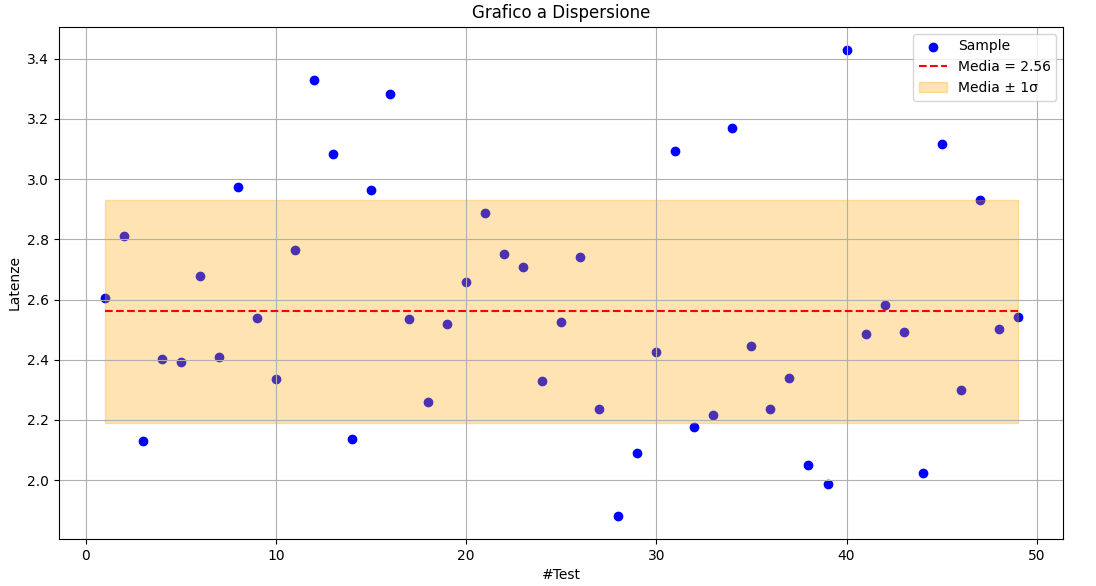
\includegraphics[width=0.9\textwidth]{figures/system-latency.png}
    \caption{Latenza totale del sistema.} 
    \label{fig:system-latency}
\end{figure}

\section{Limitazioni}

incompatibilità con le classi di confronto; dataset malformati o non disponibili;
mancanza di benchmarks e tempi di risposta(questo già visto ma ripeti bene),costi di analisi;
test manuali;
mancanza di sensoristica;